\documentclass[10pt,a4paper]{article}
\usepackage[utf8]{inputenc}
\usepackage[english,russian]{babel}
\usepackage[OT1]{fontenc}
\usepackage{amsmath}
\usepackage{amsfonts}
\usepackage{amssymb}
\usepackage{graphicx}
\usepackage{wrapfig}
\usepackage[left=1.5cm,right=1.5cm,top=1.5cm,bottom=1.5cm]{geometry}
\setlength\parindent{0pt}
\usepackage{multicol}
\usepackage{float}



\begin{document}
\begin{flushright}

\textbf{Журавлев Владимир, 621 гр.\\}

\end{flushright}
\begin{center}
\begin{LARGE}

\vspace{\baselineskip}
Лабораторная работа №4.2.1\\
\textbf{
Кольца Ньютона}\\
\vspace{\baselineskip}

\end{LARGE}
\end{center}


\section*{Цель работы}
Познакомиться с явлением интерференции в тонких пленках на примере колец Ньютона и с методикой интерференционных измерений кривизны стеклянной поверхности.
\section*{Теория}
\begin{figure}[h]
\begin{wrapfigure}{r}{0.3\textwidth}
\centering
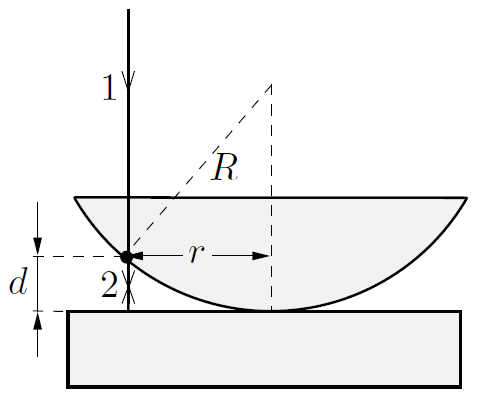
\includegraphics[width=\linewidth]{scheme.png}
\caption{Схема для наблюдения колец Ньютона в отраженном свете}
\end{wrapfigure}
Найдем толщину зазора между пластинкой и линзой из теоремы Пифагора:
\begin{equation}
R^2 = r^2 + (R-d)^2 \Rightarrow d \approx \dfrac{r^2}{2R}
\end{equation}
Разность хода между интерферирующими лучами равна
\begin{equation}
\Delta = 2d + \dfrac{\lambda}{2} = \dfrac{r^2}{R} + \dfrac{\lambda}{2}
\end{equation}
Условие интерфернционных минимумов (темных колец):
\begin{equation}
\Delta = \left(m+\dfrac{1}{2}\right)\lambda \Rightarrow r = \sqrt{m\lambda R}
\end{equation}
В этом уравнении при целых $m$ наблюдаются темные кольца, при полуцелых - светлые.
\end{figure}

\begin{figure}[h]
\begin{wrapfigure}{l}{0.5\textwidth}
\centering
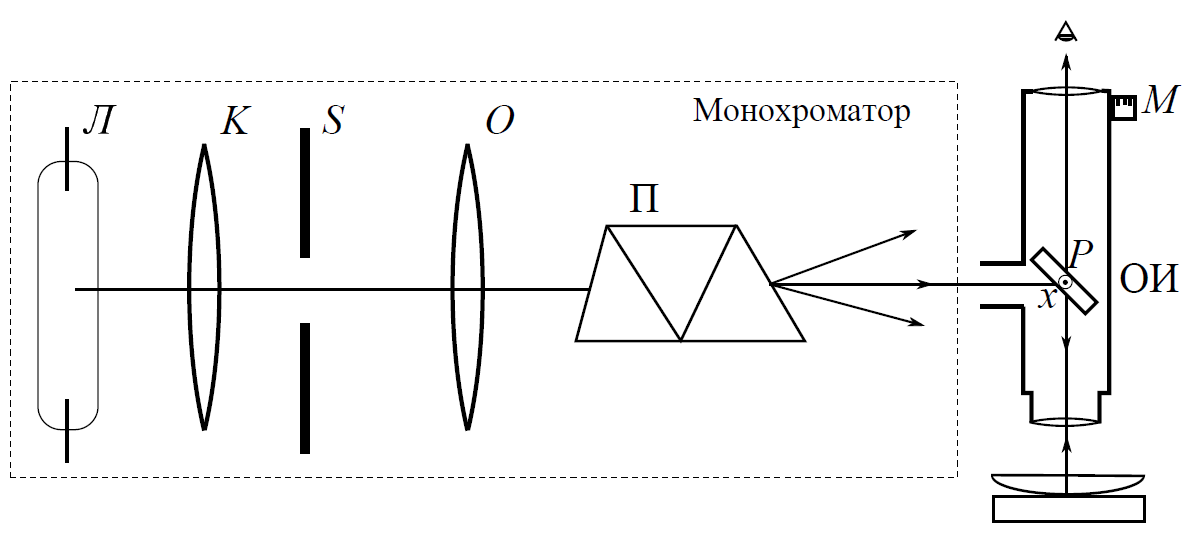
\includegraphics[width=\linewidth]{scheme1.png}
\caption{Схема установки}
\end{wrapfigure}
Если входящий пучок состоит из 2 близких линий, то наблюдаются биения - размывание видности интерференционной картины. Условие биения - наложение максимума для одной длины волны на минимум для другой:
\begin{equation}
m\lambda_1 = \left(m+\dfrac{1}{2}\right)\lambda_2 \Rightarrow \Delta\lambda = \dfrac{\lambda}{2m}
\label{oscil}
\end{equation}
\end{figure}
\clearpage
\section*{Измерения}
\subsection*{Основная часть}
Снимем зависимость радиуса темных и светлых колец от номера
\begin{table}[h]
\centering
\begin{tabular}{r|rrrrrrrrrr}\\
$n$ & $-8.0$  & $-7.5$  & $-7.0$  & $-6.5$  & $-6.0$  & $-5.5$  & $-5.0$  & $-4.5$  & $-4.0$  & $-3.5$\\
$x,\ \text{дел}$ & $0.87$  & $0.96$  & $1.06$  & $1.17$  & $1.23$  & $1.31$  & $1.4$  & $1.51$  & $1.63$  & $1.74$\\
$r,\ \text{мм}$ & $-0.228$  & $-0.220$  & $-0.211$  & $-0.202$  & $-0.196$  & $-0.189$  & $-0.181$  & $-0.171$  & $-0.160$  & $-0.151$\\
$r^2,\ \text{мм}^2$ & $0.052$  & $0.049$  & $0.045$  & $0.041$  & $0.039$  & $0.036$  & $0.033$  & $0.029$  & $0.026$  & $0.023$\\
$|n|$ & $8.0$  & $7.5$  & $7.0$  & $6.5$  & $6.0$  & $5.5$  & $5.0$  & $4.5$  & $4.0$  & $3.5$\\
\hline
$n$ & $-3.0$  & $-2.5$  & $-2.0$  & $-1.5$  & $-1.0$  & $-0.5$  & $0.0$  & $0.5$  & $1.0$  & $1.5$\\
$x,\ \text{дел}$ & $1.86$  & $2.01$  & $2.17$  & $2.34$  & $2.51$  & $2.84$  & $3.42$  & $4.02$  & $4.31$  & $4.52$\\
$r,\ \text{мм}$ & $-0.140$  & $-0.126$  & $-0.112$  & $-0.097$  & $-0.082$  & $-0.052$  & $0.000$  & $0.054$  & $0.080$  & $0.099$\\
$r^2,\ \text{мм}^2$ & $0.020$  & $0.016$  & $0.013$  & $0.009$  & $0.007$  & $0.003$  & $0.000$  & $0.003$  & $0.006$  & $0.010$\\
$|n|$ & $3.0$  & $2.5$  & $2.0$  & $1.5$  & $1.0$  & $0.5$  & $0.0$  & $0.5$  & $1.0$  & $1.5$\\
\hline
$n$ & $2.0$  & $2.5$  & $3.0$  & $3.5$  & $4.0$  & $4.5$  & $5.0$  & $5.5$  & $6.0$  & $6.5$\\
$x,\ \text{дел}$ & $4.71$  & $4.91$  & $5.05$  & $5.18$  & $5.29$  & $5.39$  & $5.49$  & $5.61$  & $5.69$  & $5.79$\\
$r,\ \text{мм}$ & $0.116$  & $0.134$  & $0.146$  & $0.158$  & $0.168$  & $0.177$  & $0.185$  & $0.196$  & $0.203$  & $0.212$\\
$r^2,\ \text{мм}^2$ & $0.013$  & $0.018$  & $0.021$  & $0.025$  & $0.028$  & $0.031$  & $0.034$  & $0.039$  & $0.041$  & $0.045$\\
$|n|$ & $2.0$  & $2.5$  & $3.0$  & $3.5$  & $4.0$  & $4.5$  & $5.0$  & $5.5$  & $6.0$  & $6.5$\\
\hline
$n$ & $7.0$  & $7.5$  & $8.0$  & $8.5$  & $9.0$  & $9.5$  & $10.0$  & $10.5$  & $11.0$  & $11.5$\\
$x,\ \text{дел}$ & $5.88$  & $5.98$  & $6.04$  & $6.12$  & $6.21$  & $6.27$  & $6.33$  & $6.4$  & $6.46$  & $6.52$\\
$r,\ \text{мм}$ & $0.220$  & $0.229$  & $0.235$  & $0.242$  & $0.250$  & $0.255$  & $0.261$  & $0.267$  & $0.272$  & $0.278$\\
$r^2,\ \text{мм}^2$ & $0.049$  & $0.053$  & $0.055$  & $0.059$  & $0.062$  & $0.065$  & $0.068$  & $0.071$  & $0.074$  & $0.077$\\
$|n|$ & $7.0$  & $7.5$  & $8.0$  & $8.5$  & $9.0$  & $9.5$  & $10.0$  & $10.5$  & $11.0$  & $11.5$\\
\hline
$n$ & $12.0$  & $12.5$  & $13.0$  & $13.5$  & $14.0$  & $14.5$  & $15.0$  & $15.5$  & $16.0$  & $16.5$\\
$x,\ \text{дел}$ & $6.61$  & $6.68$  & $6.75$  & $6.82$  & $6.91$  & $6.95$  & $7.02$  & $7.08$  & $7.14$  & $7.18$\\
$r,\ \text{мм}$ & $0.286$  & $0.292$  & $0.298$  & $0.305$  & $0.313$  & $0.316$  & $0.323$  & $0.328$  & $0.333$  & $0.337$\\
$r^2,\ \text{мм}^2$ & $0.082$  & $0.085$  & $0.089$  & $0.093$  & $0.098$  & $0.100$  & $0.104$  & $0.108$  & $0.111$  & $0.113$\\
$|n|$ & $12.0$  & $12.5$  & $13.0$  & $13.5$  & $14.0$  & $14.5$  & $15.0$  & $15.5$  & $16.0$  & $16.5$\\
\hline
$n$ & $17.0$  & $17.5$  & $18.0$  & $18.5$  & $19.0$  & $19.5$  & $20.0$ &  &  & \\
$x,\ \text{дел}$ & $7.23$  & $7.29$  & $7.34$  & $7.37$  & $7.41$  & $7.45$  & $7.49$ &  &  & \\
$r,\ \text{мм}$ & $0.341$  & $0.347$  & $0.351$  & $0.354$  & $0.358$  & $0.361$  & $0.365$ &  &  & \\
$r^2,\ \text{мм}^2$ & $0.117$  & $0.120$  & $0.123$  & $0.125$  & $0.128$  & $0.130$  & $0.133$ &  &  & \\
$|n|$ & $17.0$  & $17.5$  & $18.0$  & $18.5$  & $19.0$  & $19.5$  & $20.0$ &  &  & \\
\end{tabular}
\caption{Зависимость радиуса кольца от его номера}
\end{table}
Построим график зависимости $r^2(m)$. Угловой коэффициент прямой $\alpha = (6.85\pm0.03)\cdot 10^{-3}\ \text{мм}^2$. Найдем радиус кривизны линзы:
\begin{equation}
R = \dfrac{\alpha}{\lambda} = (11.8\pm0.1)\ \text{мм}
\end{equation}
\subsection*{Биения}
Получим биения. Для этого направим на установку 2 линии -- зеленого и желтого цвета с длинами волны $\lambda_1 = 546\ \text{нм}$ и $\lambda_2 = 577\ \text{нм}$. Количество полос между наиболее четким и наиболее размытым кольцом $\Delta m = 9\pm0.5$. Тогда по формуле (\ref{oscil}) получаем $\Delta\lambda = (31\pm2)\ \text{нм}$.

\begin{multicols}{2}


\end{multicols}

\begin{figure}[H]
\centering
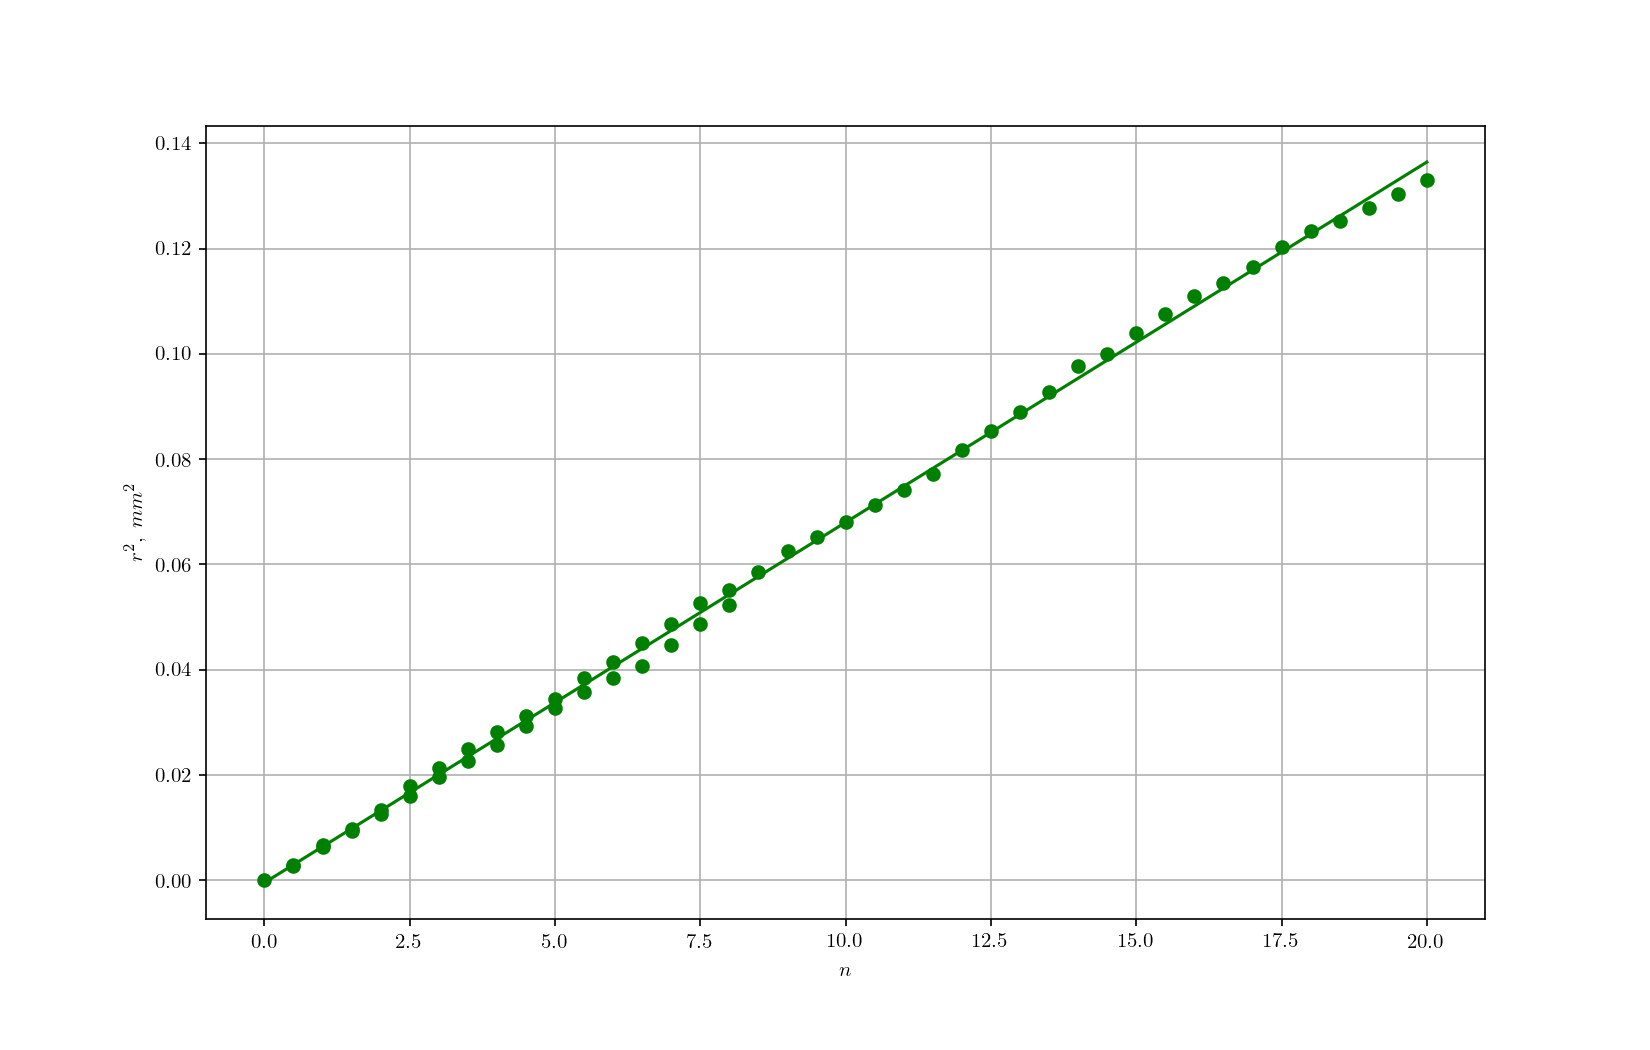
\includegraphics[width=\linewidth]{plot.png}
\caption{График зависимости радиуса колец от их номера}
\end{figure}
\subsection*{Калибровка}
0 деление шкалы видно при $x_1 = 0.17\ \text{дел}$, 75 -- при $x_2 = 8.54\ \text{дел}$. Отсюда с учетом того, что у шкалы $100\ \text{дел} = 1\ \text{мм}$, получаем $1\ \text{дел} = 89.6\ \text{мкм}$.


\section*{Выводы}
\begin{itemize}
\item Получена интерференционная картина колец Ньютона
\item Измерена зависимость радиуса колец от их номеров
\item Вычислен радиус кривизны линзы $R = (11.8\pm0.1)\ \text{мм}$
\item Получена картина биений для двух близких длин волн, вычислена разность $\Delta\lambda = (31\pm2)\ \text{нм}$. У ртутной лампы зеленая линия имеет длину волны $\lambda_1 = 546\ \text{нм}$, желтая -- $\lambda_2 = 577\ \text{нм} \Rightarrow \lambda_2-\lambda_1 = 31\ \text{нм}$. Таким образом полученные данные находятся в согласии с теорией.
\end{itemize}



\end{document}